\documentclass{beamer}
\usepackage{verbatim}
\usepackage[usenames]{color}

\title{ADAM:  Analysis of Discrete Models of Biological Systems Using Computer Algebra}
\author{Bonny Guang, Madison Brandon, Rustin McNeill}
\date{August 6th, 2010}

\begin{document}

\maketitle

\begin{frame}
Why use models in Biology?
\begin{itemize}
	\item{In biological systems, concerned with how different elements in the system interact with one another.}
	\item{One way to describe such interactions: create a model which describes the system.}
	\item{Can be either quantitative or qualitative descriptions, or both.}
	\item{One can obtain relevant information about system from models without having to perform costly experiments.}
\end{itemize}
\end{frame}


\begin{frame}
	\frametitle{Discrete vs. Continuous Models}
	\begin{center}
	\begin{itemize}
	  \item{Simple Model of Population Growth}
		\item{Given $P_0=1$, $r=0.5$, and $K=100$.}
	\end{itemize}
	\end{center}
	\begin{columns}
    \begin{column}[l]{0.5\textwidth}
    Discrete\\$P_t = P_t + rP_t$, $t=0,1,2,3$
    \begin{figure}
		  \includegraphics[width=2.5in,height=1.5in]{discreteEx.jpg}
		\end{figure}
    \end{column}
    \begin{column}[r]{0.5\textwidth}
    Continuous\\$\frac{dP}{dt} = rP(1-\frac{P}{K})$, $t\in[0,3]$
    \begin{figure}
		  \includegraphics[width=2.5in,height=1.5in]{continuousEx.jpg}
		\end{figure}
    \end{column}
  \end{columns}	  
\end{frame}

\begin{frame}
	\frametitle{Models in Biology}
	\begin{columns}
	\begin{column}[l]{0.5\textwidth}
	Continuous Models:	
		\begin{itemize}
			\item{Rely on exact parameter rates}
			\item{Often not intuitive}
			\item{Many tools available for analysis}
		\end{itemize}
	\end{column}
	\begin{column}[r]{0.5\textwidth}
	Discrete Models:
		\begin{itemize}
			\item{Finite number of states}
			\item{Intuitive}
			\item{Few mathematical tools available for analysis}
		\end{itemize}
	\end{column}
	\end{columns}
	\begin{figure}
		\centering
		\includegraphics[scale = 0.35]{Model_diagram.png}
%		\caption{Diagram representing different types of models used in biology along with examples of corresponding analytic software.}
	\end{figure}
\end{frame}

\begin{frame}
 \frametitle{Applications of Discrete Models}
  \begin{figure}
 		\centering
		\includegraphics[width=3.6in,height=0.7in]{signalingNetworks_pdf.png}
		\end{figure}
  \begin{figure}
 		\centering
		\includegraphics[width=3.6in,height=0.9in]{glucose_pdf.png}
	\end{figure}	
  \begin{figure}
 		\centering
		\includegraphics[width=3.6in,height=1.1in]{petriNet_pdf.png}
		\end{figure}	
\end{frame}

\begin{frame}
	\frametitle{Key Dynamical Features}
	\begin{columns}
  	\begin{column}[l]{0.5\textwidth}
		\begin{figure}
			\centering
			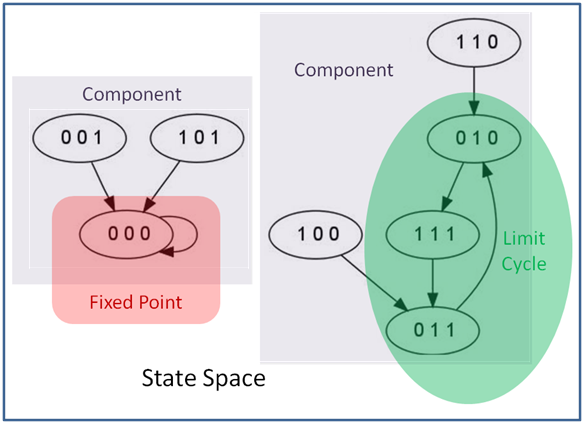
\includegraphics[height=1.5in,width=2in]{state_space_poster.png}
			\caption{Example State Space}
		\end{figure}
		\end{column}
		\begin{column}[r]{0.5\textwidth}
		\begin{itemize}
 			\item{\textcolor{red}{Fixed Point} - may give researcher info about what combination of gene states leads to permanently fixed state.}
 			\item{\textcolor{green}{Limit Cycle} - limit cycles and their length can indicate recurring processes in the cell cycle.}
 			\item{\textcolor{purple}{Component} - typically modeler expects small limit cycles with large component sizes.}
 		\end{itemize}
		\end{column}
	\end{columns}
\end{frame}	

\begin{frame}
	\frametitle{Simple Example}
\begin{columns}
  \begin{column}[l]{0.5\textwidth}
	\begin{figure}
		\centering
		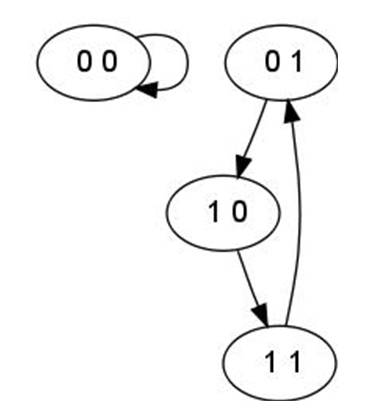
\includegraphics[height=1in,width=1in]{2by2Ex_statespace.jpg}
		\caption{State space for a 2 by 2 system}
	\end{figure}
	\end{column}
	
	\begin{column}[r]{0.5\textwidth}
	\begin{figure}
 		\centering
		\includegraphics[height=1in,width=2in]{2by2Ex_table.jpg}
		\caption{Truth table for 2 by 2 system}
	\end{figure}
	\end{column}
\end{columns}
\end{frame}

\begin{frame}
	\frametitle{Simple Example}
	\vspace{-20pt}
	\begin{figure}
	\centering
		\includegraphics[height=1.2in,width=1.75in]{boolfunction.png}
	\end{figure}
	Can write any boolean function defined this way as polynomial $f:\mathbb{F}_2^2\rightarrow\mathbb{F}_2^2$ where\\
	\begin{equation*}
		 f_1(x1,x2) = \sum_{i=1}^4 b_i \prod_{j=1}^2 (1 - (c_{i,j} - x_i))
	\end{equation*}\\
	where $c_{i,j}$ are the $i,j$th entries into the matrix {\color{red}$C$} and $b_i$ are the $i$th entries into the vector {\color{blue}$B$}.\\
\end{frame}

\begin{frame}
	\frametitle{Simple Example}
	Then
	\begin{align*}
	f_1 &= 0*(1-(0-x_1)(1-(0-x_2)) \\
	&+ 1*(1-(0-x_1))(1-(1-x_2)) \\
	&+ 1*(1-(1-x_1))(1-(0-x_2)) \\
	&+ 0*(1-(1-x_1))(1-(1-x_2))\\ \\
	&= (1-x_1)x_2 + x_1(1-x_2)\\ \\
	&= x1+x2\\ 
	\end{align*}
	This is a polynomial in $\mathbb{F}_2^2$.
\end{frame}


%%%%%%%%%%%%%%%%%%%%%%%%%%%%%%%%%%%%% begin Lambda Phage Example  %%%%%%%%%%%%%%%%%%%%%%%%%%%%%%%%
\begin{frame}
	\frametitle{Lambda Phage Example}
	\begin{itemize}
	\item Lambda phage is virus that hijacks host cell
	\item Viral reproduction process shown below is called the Lysogenic Cycle.
	\end{itemize}
	\begin{columns}
  	\begin{column}[l]{0.5\textwidth}
		\begin{figure}
			\centering
			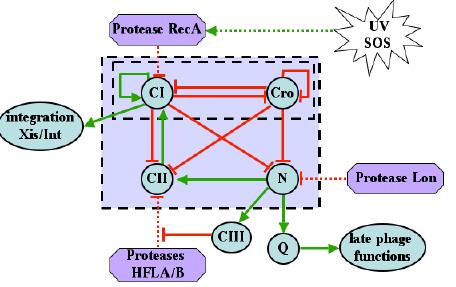
\includegraphics[height=1.5in,width=2in]{phageWD.jpg}
			\caption{Logical model of lysogenic cycle by Lambda Phage virus}
		\end{figure}
		\end{column}
		\begin{column}[r]{0.5\textwidth}
		\begin{itemize}
 			\item{Red arrows signify inhibition.}
 			\item{Green arrows signify activation.}
 			\item{Ex: CII activates CI; CI maintains its own expression while repressing CII, Cro, and N.}
 		\end{itemize}
		\end{column}
	\end{columns}	
\end{frame}

\begin{frame}
 \frametitle{Lambda Phage Example}
\begin{columns}
\begin{column}{0.5\textwidth}
\begin{itemize}
  \item{State written as vector with four entries: (CI,CII,Cro,N)}
  \item{Genes have 5 possible values; hence $5^4$ $=$ 625 states.}
  \item{State (1,0,0,3) means concentration of CI is low, genes CII and Cro are off, and N is medium.}
  \item{$f_i$ determines state of the gene represented by $x_i$.}
  \item{Ex: $f_{C1} = -2x_{Cro}^{4}+2$ in means $x_{C1}$ is 0 or 2 based on $x_{Cro}$.}
\end{itemize}
\end{column}
\begin{column}{0.5\textwidth}
   \begin{figure}
 		  \centering
		  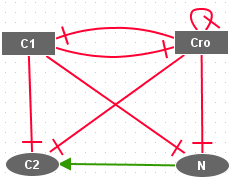
\includegraphics[width=1.50in]{PHAGE4nice.png}
   \end{figure}
\pause
   \begin{table}
     \begin{tabular}{| l | r |}
\hline
$x_{Cro}$ & $f_{C1}$ \\ \hline
0 & 2 \\
1 & 0 \\
2 & 0 \\
3 & 0 \\
4 & 0 \\
\hline
     \end{tabular}
   \end{table}
\end{column}
\end{columns}
\end{frame}

\begin{frame}
	\frametitle{Lambda Phage Example}
	\begin{itemize}
	\item Lambda phage model can be uploaded to ADAM for analysis.
	\item ADAM will output PDS from truth table with corresponding variable descriptions.
	\item ADAM will also output analysis of dynamics.
	\end{itemize}
	\begin{figure}
		\centering
		\includegraphics[height=1in,width=3.1in]{ADAMss_simoutput.png}
		\caption{Output from ADAM for analysis of lambda phage}
	\end{figure}
	\begin{itemize}
	\item One fixed point at (2,0,0,0)
	\item Two limit cycles
	\end{itemize}
\end{frame}

%%%%%%%%%%%%%%%%%%%%%%%%%%%%%%%%%% end Lambda Phage Example  %%%%%%%%%%%%%%%%%%%%%%%%%%%%%

%%%%%%%%%%%%%%%%%%%%%%%%%%%%%%%%%% begin Large Systems  %%%%%%%%%%%%%%%%%%%%%%%%%%%%%%%%%%%

\begin{frame}
 \frametitle{What Happens as the System Gets Larger?}
\begin{figure}
    \vspace{-10pt}
    \caption{Mammalian cell cycle with at least 60 nodes.}
    \centering
    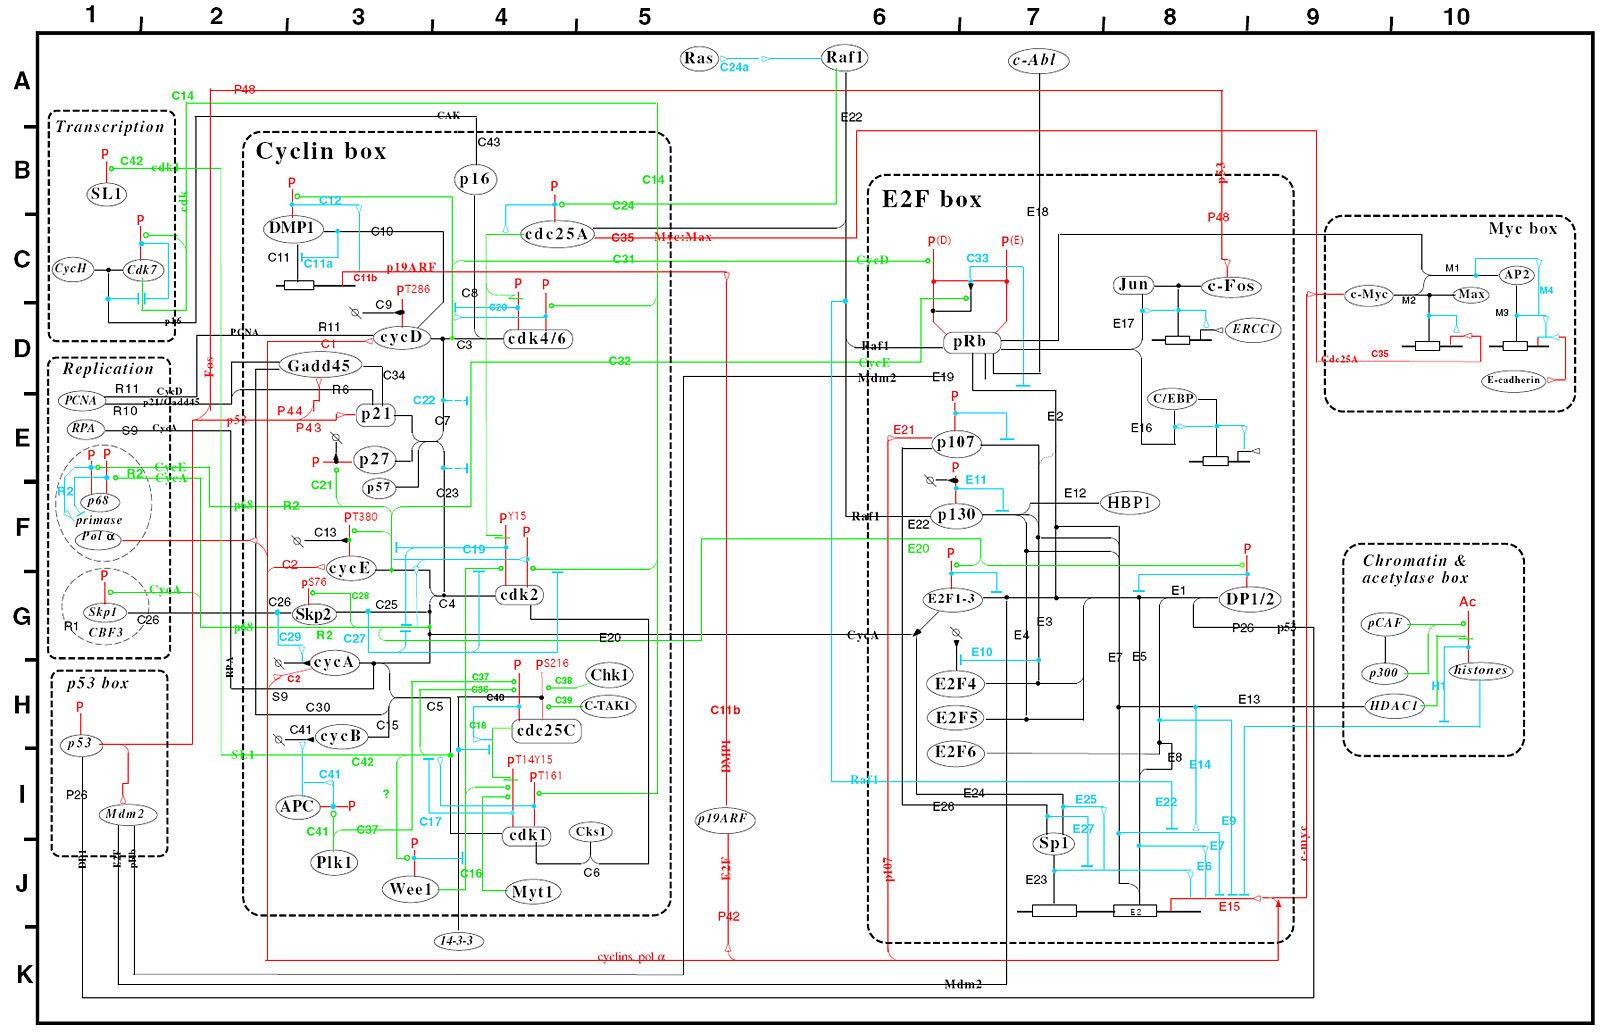
\includegraphics[width = 0.95\textwidth]{hugewiringdiagram.jpg}
    \vspace{-10pt}
\end{figure}
\end{frame}

\begin{frame}
 \frametitle{State Space Diagrams}
\begin{itemize}
 \item $2^{60} \approx 1,200,000,000,000,000,000$ states. Let's scale down to $n = 9$ nodes. (ADAM only allows simulation up to 11 nodes)
 \item Even for $n = 9$, when we try to see the state space graph...
\end{itemize}
\pause \begin{figure}
    \caption{Boolean state space graph, 9 nodes.}
    \centering
    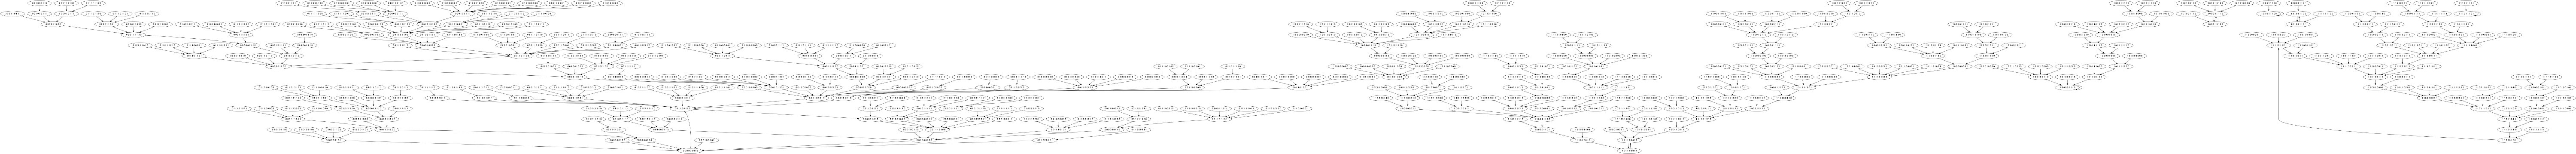
\includegraphics[width = 4in]{9states-1.jpg}
\end{figure}
Impossible to even see the states on one screen!
\pause \begin{figure}
    \caption{Cropping of 3\% of graph}
    \centering
    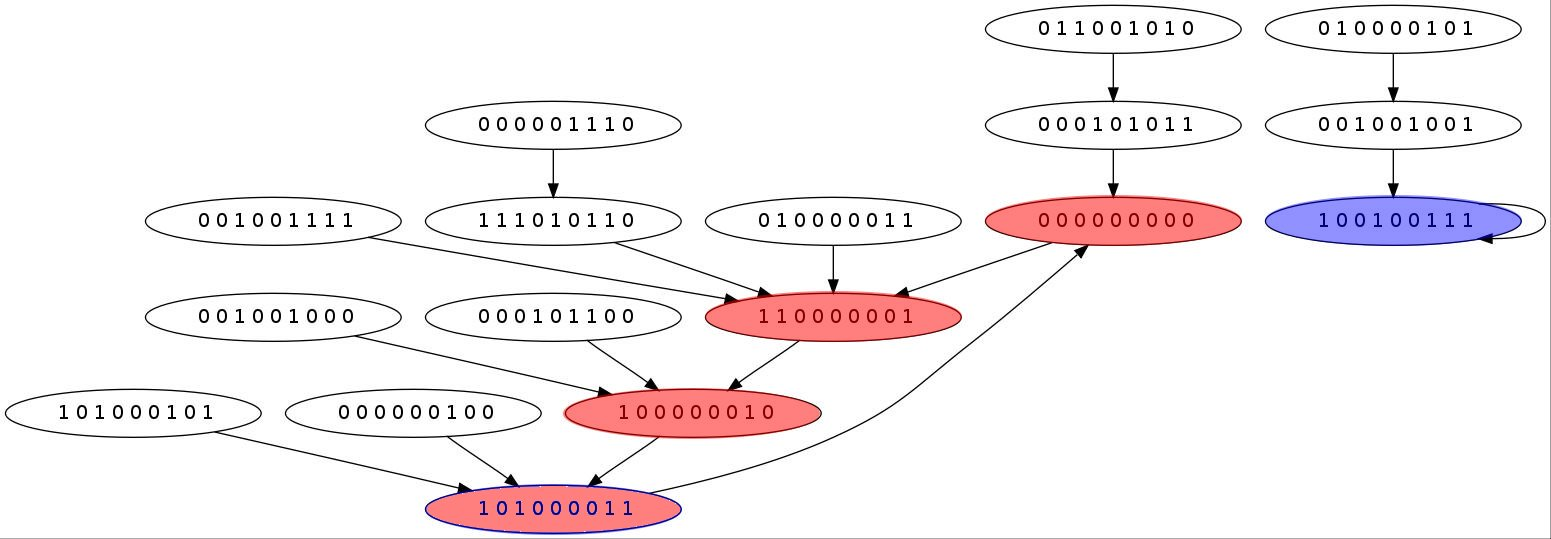
\includegraphics[width = 0.7\textwidth]{RandomNetwork.jpg}
\end{figure}
\end{frame}

\begin{frame}
\frametitle{Why simulation isn't enough}
How many states can a biological system have?\\ 
\vspace{5mm}
Network controlling ErBb2 regulation: 17 nodes, off, low or high \\
\begin{itemize}
\item{$3^{17} = 129,140,163$}
\end{itemize}
\vspace{2mm}
Mamillian Cell Cycle: 60 nodes, on or off
\begin{itemize}
\item{$2^{60} = 1,152,921,504,606,846,976$}
\end{itemize}
\vspace{2mm}
Budding Yeast Cell Cycle: 27 nodes, off, low or high
\begin{itemize}
\item{$3^{27} = 7,625,597,484,987$}
\end{itemize}
\end{frame}

%%%%%%%%%%%%%%%%%%%%%%%%%  end Large Systems %%%%%%%%%%%%%%%%%%%%%%%%%%%%%%%%%


%%%%%%%%%%%%%%%%%%%%%%%%%  begin Benchmarking Slides   %%%%%%%%%%%%%%%%%%%%%%%%%%%%%%%%%%

\begin{frame}
	\frametitle{Searching for an Alternative to Simulation}
	\begin{itemize}
		\item{In biological systems, input generally only comes from a few nodes.}
		\item{In gene regulatory networks genes are regulated by only a handful of regulators.}
		\item{Hence PDSs representing such biological networks are sparse.}
		\item{We compute the Gr\"obner basis of the PDS to simplify analysis.}
		\item{Computations are fast because sparse structure is preserved by Gr\"obner basis.}
	\end{itemize}	
\end{frame}

\begin{frame}
	\frametitle{Benchmark Test Results}
	Based on benchmark tests on algorithms which compute fixed points, showed that algorithms particularly fast on large sparse systems. 	All benchmark tests run on a 2.27 GHz processor. 
	\begin{figure}
  \begin{center}
    \begin{minipage}[h]{0.58\linewidth}
      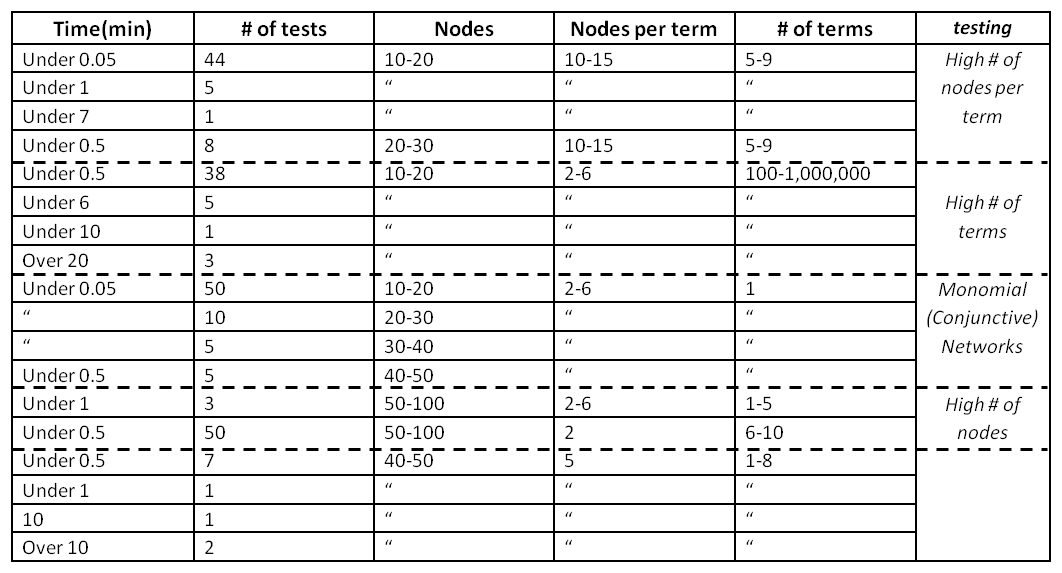
\includegraphics[scale=.37]{benchmarkTable.png}
    \end{minipage}\hfill
    \begin{minipage}[h]{0.38\linewidth}
      \caption{Benchmark tests run on randomly generated Boolean functions with different ranges of variables, terms per function, and 			 			maximum of variables per term.}
    \end{minipage}
  \end{center}
	\end{figure}		
	91 \% of computations completed in less than 30 seconds.
\end{frame}

\begin{frame}
	\frametitle{GINsim Benchmark Tests}
	\begin{figure}
 		\centering
 		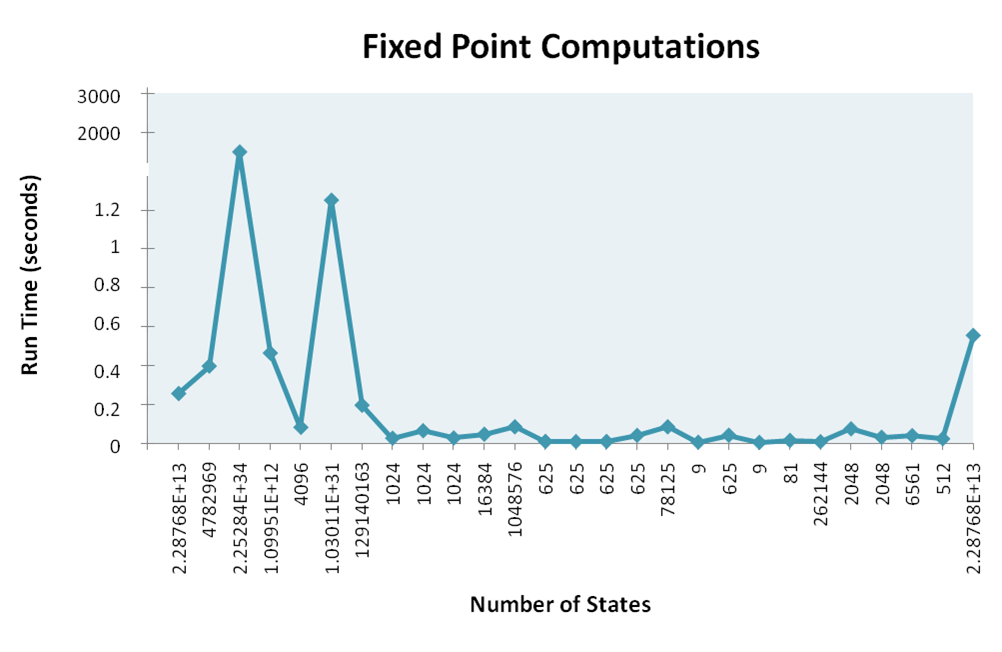
\includegraphics[scale=.33]{GINsimFP.png}
		\caption{Plot representing run times for fixed point calculations done on 25 logical models.  The number of nodes in each file ranges from 2 to 72.}
	\end{figure}
\end{frame}

\begin{comment}
\begin{frame}
	\frametitle{GINsim Benchmark Tests}
	\begin{itemize}
		\item{27 GINsim files from the model repository tested}
		\item{Average number of nodes: 14}
		\item{Average time to compute all fixed points of a system: 0.15 seconds}
		\item{Biological system with the most nodes: 65}
		\begin{itemize}	
			\item{Th cell differentiation model}
			\item{3 states (0, 1, 2)}
			\item{1.25 seconds to find the three fixed points}
		\end{itemize}
		\item{Outlier:}
		\begin{itemize}
			\item{Segment Polarity}
			\item{72 nodes, 3 states}
			\item{18 minutes to find 65 fixed points}
			\item{$2.34 \cdot 10^{34} states$}
		\end{itemize}
		\item{Longest limit cycle: one 7-cycle present}
		\item{Calculated 20 cycles for 14 systems}
	\end{itemize}
\end{frame}
\end{comment}

%%%%%%%%%%%%%%%%%%%%%%%%% end Benchmarking Slides   %%%%%%%%%%%%%%%%%%%%%%%%%%%%%%%%%%%%%


%%%%%%%%%%%%%%%%%%%%%%%%% begin ADAM description  %%%%%%%%%%%%%%%%%%%%%%%%%%%%%%%%%%
\begin{frame}
 \frametitle{ADAM:  Analysis of Discrete Algebraic Models}
\begin{itemize}
  \item{Analogy: MatLAB - solves continuous models such as ODEs - does not require understanding of ODE solvers.}
  \item{ADAM analyzes discrete models by a combination of simulation and algorithms - does not require understanding of underlying mathematics.}
  \item{ADAM can analyze: 
  	\begin{itemize}
  		\item{\textbf{Logical Models}(in GINSim format)}
  		\item{\textbf{Polynomial Dynamical Systems (PDS)}}
  		\item{\textbf{Probabilistic Boolean (or multistate) Networks}}}
		\end{itemize}
	\item{$<$http://dvd.vbi.vt.edu/cgi-bin/git/adam.pl$>$}
\end{itemize}
\end{frame}

\begin{frame}
\frametitle{Meet ADAM:  \small{$<$http://dvd.vbi.vt.edu/cgi-bin/git/adam.pl$>$}}
\begin{center}
\includegraphics[scale=.45]{ADAMss_phage4.png}
\end{center}
\end{frame}

%%%%%%%%%%%%%%%%%%%%%%%%% end ADAM description %%%%%%%%%%%%%%%%%%%%%5



%%%%%%%%%%%%%%%%%%%%%%%%%%%%%%%%  TCR example  %%%%%%%%%%%%%%%%%%%%%%%%

\begin{frame}
\frametitle{TCR Signalization Pathway}

\begin{itemize}

	\item{Boolean logical model with 40 nodes $\rightarrow 2^{40} = 1,099,511,627,776$ states}
	\item{For a state space this large simulation is inefficient}
\end{itemize}
Using ADAM: \\
\begin{itemize}
	\item{fixed point analysis $<$ .5 seconds}
	\item{analyzed limit cycles up to length 20 with a total runtime $<$ 1 minute}
	\item{finds a limit cycle which was not found in the published analysis}
\end{itemize}
\begin{center}
\includegraphics[scale=.4]{TCR7-cycle.png}
\end{center}
\end{frame}



%%%%%%%%%%%%%%%%%%%%%%%%%%%%%%%%%%%%%%%%%%%%%%%%%%%%%%%%%%%%%%%%%%%%%%%%%

%\begin{frame}
%	\frametitle{Recap}
%	\begin{figure}
% 		\centering
%		\includegraphics[width=4.6in]{flowchart_fixed.png}
%	\end{figure}
%\end{frame}


\begin{frame}
\frametitle{Conclusions}

\begin{itemize}
	\item{Discrete Modeling techniques useful tool for \textbf{analyzing biological systems}}
	\item{Can analyze discrete models, i.e. logical networks, petri-nets, or agent-based models, by \textbf{converting into polynomial dynamical systems (PDS)}}
	\item{Once these models have an algebraic structure, use \textbf{tools from computational algebra to compute key dynamics}.}
	\item{Algorithms we developed are \textbf{fast for sparse systems}, a structure maintained by most biological systems}
	\item{All algorithms included in \textbf{user-friendly and free software package ADAM}}
\end{itemize}
\end{frame}


\begin{frame}
	\frametitle{Future Developments}
ADAM can be extended to...
	\begin{itemize}
		\item{Include better visualization for larger networks}
		\item{Incorporate into other software packages like Polynome or GINsim}
		\item{Automatic conversion for other model types such as petri nets}
		\item{Implement analytic methods/algorithms to reduce computational complexity and improve efficiency}
	\end{itemize}
\end{frame}

\begin{frame}
	\frametitle{Acknowledgements}
This research was conducted during the Research Experience for Undergraduates (REU), Modeling and Simulation in Systems Biology (MSSB) at 		Virginia Bioinformatics Institute (VBI), Virginia Tech University.  This research was funded by the National Science Foundation, fund number  0755322.

	\begin{columns}
		\begin{column}{0.33\textwidth}
		\begin{figure}
 			\centering
			\includegraphics[scale=.2]{VBIlogo.png}
		\end{figure}
		\end{column}
		\begin{column}{0.33\textwidth}
		\begin{figure}
 			\centering
			\includegraphics[scale=.2]{Techlogo.png}
		\end{figure}
		\end{column}
		\begin{column}{0.33\textwidth}
		\begin{figure}
 			\centering
			\includegraphics[scale=.3]{NSFlogo.png}
		\end{figure}
		\end{column}
	\end{columns}
\end{frame}

\begin{comment}
\begin{frame}
\begin{thebibliography}{5in}
\tiny
	\bibitem{Abdul:2008} Abdul Salam Jarrah, Reinhard Laubenbacher, Alan Veliz-Cuba, (2008) The Dynamics of Conjunctive and Disjunctive Boolean Network Models. \textit{Bioinformatics}.
	\bibitem{ADAM} \textit{ADAM Home}. <http://dvd.vbi.vt.edu/cgi-bin/git/adam.pl>.
	\bibitem{Aur�lien:2007} Aur�lien Naldi, Denis Thieffry, and Claudine Chaouiya. (2007) Decision Diagrams for the Representation and
Analysis of Logical Models of Genetic Networks. \textit{Computer Science}.
	\bibitem{Brown:1971} Brown W.S. (1971) On Euclid's Algorithm and the Computation of Polynomial Greatest Common Divisors. \textit{Journal of the ACM}.
	\bibitem{GINsim} \textit{GINsim Home}. <http://gin.univ-mrs.fr/>.
  \bibitem{Hinkelmann:2010} Hinkelmanna, Franziska, Murrugarraa, David, Jarrahb, Abdul Salam, Laubenbacher, Reinhard. (2010) A Mathematical Framework for Agent Based Models of Complex Biological Networks. \textit{Quantitative Biology}. 
  \bibitem{Leclerc:2008} Leclerc, Robert D. (2008) Survival of the Sparsest: Robust Gene Networks are Parsimonious. \textit{Ecology and Evolutionary Biology}.
  \bibitem{Lidl:1997} Lidl, R., Niederreiter, H., 1997. Finite Fields, Encyclopedia of Mathematics and its Applications 20, 2nd Edition. Cambridge University Press, Cambridge.
	\bibitem{Macaulay2} \textit{Macaulay2 Home}. Grayson, Daniel R. and Stillman, Michael E.  Macaulay2, a software system for research in algebraic geometry.  Available at <http://www.math.uiuc.edu/Macaulay2/>.
	\bibitem{polynome} \textit{Polynome}. <http://polymath.vbi.vt.edu:3002/>.
	\bibitem{Remy:2005} Remy E., Ruet P., Thieffry D., (2005) Graphic Requirements for Multistability and Attractive Cycles in a Boolean Dynamical Framework. Advances in Applied Mathematics Volume 41, Issue 3, September 2008, Pages 335-350. 
	\bibitem{TCR} \textit{TCR Signalisation Pathway}. 	<http://gin.univ-mrs.fr/GINsim/model$_$repository/MAMMALIAN\_REGULATORY
\_NETWORKS/T\_lymphocytes/TCR\_sig/description.html>.
	\bibitem{Thomas:2001} Thomas R., (2001) Kaufman M., Multistationarity, The Basis of Cell Differentiation and Memory. I. Structural Conditions of Multistationarity and Other Nontrivial Behaviour. Chaos, Vol. 11, pp. 170-179.
	\bibitem{Ting:1999} Ting Chen, Hongyu L. He, George M. Church. (1999) Modeling Gene Expressions with Differential Equations. \textit{Genetics}.
	\bibitem{Veliz-Cuba:2010} Veliz-Cuba A., Salam Jarrah A., Laubenbacher R., (2010) Polynomial Algebra of Discrete Models in Systems Biology. \textit{Bioinformatics}.
\end{thebibliography}
\end{frame}
\end{comment}

\end{document}
